\documentclass[10pt]{article}
\usepackage[a5paper, margin=1cm]{geometry}
\usepackage{concmath} %palatino} %mlmodern
% \usepackage{lipsum} %for sample text
\usepackage{tikz}
\usetikzlibrary{shadings,shapes,shadows}


\title{\Huge TikZ by \textit{KAZ}}
\date{\small December 30, 2024}

\begin{document}

% \lipsum[1] %sample text
\maketitle

\section*{Table}
\begin{center}
\begin{tabular}{l | c | c | c}
\hline
\hline \textbf{Name} & \textbf{ID} & \textbf{Year} & \textbf{Hall} \\
\hline Debashish & 23701034 & 2nd & A Hall \\
\hline Miskat & 23701052 & 2nd & A Hall \\
\hline Sabrina & 23701072 & 2nd & B Hall \\
\hline Sumaiya & 23701025 & 2nd & B Hall \\
\hline \hline
\end{tabular}
\end{center}


\section*{Drawing shapes}
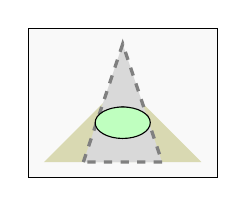
\begin{tikzpicture}
    \draw[fill=gray!5] (0.8,0.8) rectangle (3.2,2.7);
    
    \path[fill=green!50!red!30] (1,1) -- (2,2) -- (3,1) -- cycle; %cycle to connect the points
    
    \path[draw=gray,very thick, style=dashed,fill=gray!30] (1.5,1) -- (2,2.5) -- (2.5,1) -- cycle; %here draw=gray draws the outline of the inside triangle

    \draw[fill=red!25] (2,1.5) circle (0.2);

    \draw[fill=green!25] (2,1.5) ellipse (0.35 and 0.2);    
\end{tikzpicture}\newline



\section*{Connecting node like a triangle}
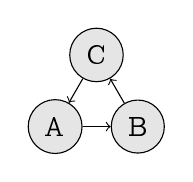
\begin{tikzpicture}[scale=0.7]
    \node[circle,draw,fill=gray!20] (a) at (0,0) {A};
    %\path[draw, fill=gray!20] (0,0) node[circle] {A};
    \node[circle,draw,fill=gray!20] (b) at (0:1.5) {B}; % (angle:distance), here : is used while considering angle
    \node[circle,draw,fill=gray!20] (c) at (60:1.5) {C};
    \draw[->] (a) -- (b);
    \draw[->] (b) -- (c);
    \draw[->] (c) -- (a); 
\end{tikzpicture}\\



\section*{Using loop to draw multiple nodes}
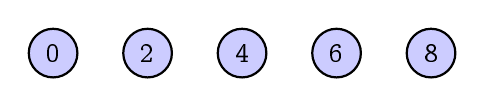
\begin{tikzpicture}[scale=0.6]
    \foreach \n in {0, 2, ..., 9}  \node[circle,draw=black,thick,fill=blue!20] at (\n,0) {\n};
\end{tikzpicture}\\ 



\section*{Connect circular nodes with arrows from centre}
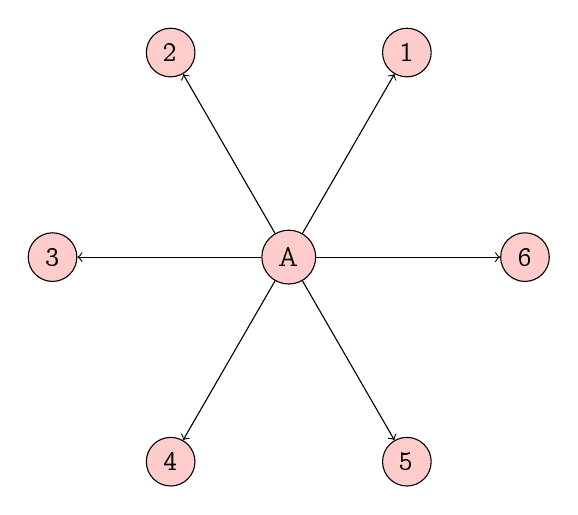
\begin{tikzpicture}
    %central node
    \node[circle,draw,fill=red!20] (a) at (0,0) {A}; 
    \foreach \n in {1, 2, ..., 6} \node[circle,draw,fill=red!20] (\n) at (60*\n:3) {\n};
    \foreach \n in {1, 2, ..., 6} {
        \draw[->] (a) -- (\n); % Arrows from central node (a) to each other node
    }    
\end{tikzpicture}



\section*{Connect circular nodes with arrows as a circle}
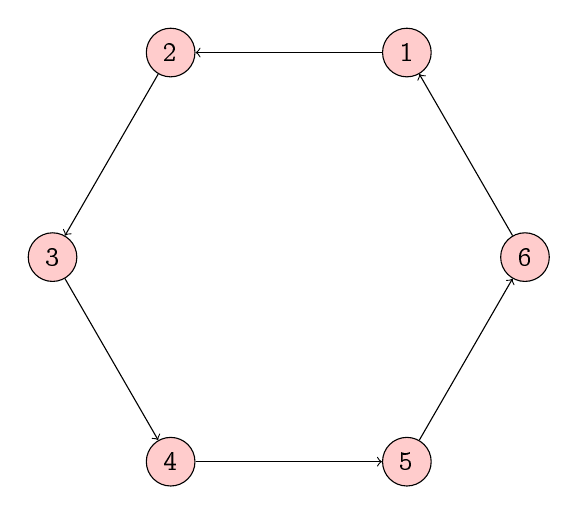
\begin{tikzpicture}
    \foreach \n in {1, 2, ..., 6} \node[circle,draw,fill=red!20] (\n) at (60*\n:3) {\n};
    \foreach \n [count=\next from 2] in {1, 2, ..., 6} {
        \ifnum\n=6
            \break % Fake "break" (prevents further drawing but technically still iterates)
        \else
            \draw[->] (\n) -- (\next);
        \fi
    }
    % Manually connect last node back to first
    \draw[->] (6) -- (1);   
\end{tikzpicture}


\end{document}

\section*{Drawing a tree}
\begin[tikzpicture}
	[every node /. style = {circle, draw],
	level 1/. style = {sibling distance = 50mm},
	level 1/. style = {sibling distance = 20mm},
	level 1/. style = {sibling distance = 10mm}]
	\node{A}
		 child {node {B}
 		  child{node{D}
 			child{node{1}}
 			child{node{2}}
 		}
 child{node {E}
 child{node{3}}
 child{node{4}}
 }
 }
 child {node(1) {C}
 child{node{F}
 child{node{5}}
 child{node{6}}
 }
 child{node{G}
 child{node{7}}
 child{node{8}}
 }
\end{tikzpicture}
